\documentclass[fontsize=10px, a4paper, openany]{scrbook}
\usepackage[left=2cm,right=1.5cm,top=2cm,bottom=3cm,bindingoffset=0cm]{geometry}
%\usepackage{ucs}
\usepackage{amsmath}
\usepackage{amssymb}
\usepackage[utf8x]{inputenc}
\usepackage[russian]{babel}
\usepackage{hyperref}
\usepackage{graphicx}
\usepackage{parskip}
\usepackage[dvipsnames,table,xcdraw]{xcolor}
\usepackage{listings}
\lstset{language=Java} 

\addtokomafont{title}{\ttfamily\flushright}
\addtokomafont{date}{\ttfamily\flushright}
\addtokomafont{chapter}{\ttfamily\bfseries}
\addtokomafont{section}{\ttfamily}
\definecolor{light-gray}{gray}{0.9}

\newcommand{\mypath}[1]{\colorbox{Apricot}{\texttt{#1}}}
\newcommand{\codeline}[1]{\vspace{5px}\colorbox{light-gray}{\texttt{#1}}\vspace{5px}}
\newcommand{\myalert}[1]{\par\vspace{5px}\noindent\fbox{#1}\vspace{5px}\par}
\newcommand{\myarr}{$\rightarrow$ }
\setlength{\parskip}{5px}
\lstset{backgroundcolor=\color{light-gray},basicstyle=\footnotesize\ttfamily,numbers=left}

\author{}
\title{Sch3dedit -- программа для построения и создания 3D-моделей стереометрических чертежей.\\Пособие для разработчиков.}
\date{\today}

\begin{document}
\maketitle
\tableofcontents
\chapter*{Введение}
\addcontentsline{toc}{chapter}{Введение}

\section*{Описание}
\texttt{3D-SchoolEdit} --- программа для создания геометрических и стереометрических чертежей с возможностью их дальнейшего экспорта в 3D-модели. Разработка ведётся на Java 7, для десктопной версии интерфейс реализован на платформе Java Swing. Приложение позиционируется как кроссплатформенное, но ориентировано, в первую очередь, на пользователей \texttt{Windows 7 / 8 / 10}.

\section*{Установка и настройка рабочего окружения}
\addcontentsline{toc}{section}{Установка и настройка рабочего окружения}
\begin{enumerate}
\item Платформа JDK 7 --- скачать и установить можно \href{http://www.oracle.com/technetwork/java/javase/downloads/jdk7-downloads-1880260.html}{отсюда}, либо

\codeline{sudo apt-get install openjdk-7-jdk}

на Linux.

Убедитесь, что сборка выполняется на правильной версии платформы.

По умолчанию JDK устанавливается в папку \mypath{C:\textbackslash Program Files\textbackslash Java}.
Путь к JDK желательно прописать в нетбинсовском конфиге: \mypath{C:\textbackslash Program Files\textbackslash NetBeans 8.0\textbackslash etc\textbackslash netbeans.conf} (путь по умолчанию)

Ключ \texttt{netbeans\_jdkhome}:

\codeline{netbeans\_jdkhome="C:\textbackslash Program Files\textbackslash Java\textbackslash jdk1.7.0\_79}

(версии JDK и NetBeans могут отличаться)

\item Maven (для работы из \href{#}{консоли}: установка хорошо описана \href{https://habrahabr.ru/post/77382/}{здесь}.

Поскольку большинство IDE имеют встроенную поддержку работы с Maven, то для начала работы достаточно просто открыть проект (NetBeans) или сделать импорт проекта (Intellij IDEA). Все зависимости скачаются автоматически.

\myalert{Следующие установки только для NetBeans.}

\item Настройки форматирования кода (для NetBeans) содержатся в файле \href{http://corp7.uniyar.ac.ru:7416/redmine/attachments/download/161/formatting\_options.zip}{ссылка}

Применяем настройки из файла \mypath{formatting\_options.zip}:

\codeline{Tools \myarr Options \myarr Import$\ldots$}

Ставим все галочки.

\item Установка русского Spellchecker (чтобы русские комментарии не подчёркивались красным). Скачиваем файл с модулем \href{http://corp7.uniyar.ac.ru:7416/redmine/attachments/download/166/netbeans-modules-spellchecker-dictionary_ru.nbm}{отсюда}. 

\codeline{Tools \myarr Plugins \myarr Downloaded \myarr Add Plugins$\ldots$}

Заходим в настройки плагина:

\codeline{Tools \myarr Options \myarr Editor \myarr Spellchecker}

Ставим \texttt{Default locale} в \texttt{ru}. Теперь нужно что-нибудь напечатать в любом файле и сохранить. Через несколько минут словарь закэшируется и будет работать.

\item Меняем стандартные настройки профайлера: \texttt{Connection Timeout} по умолчанию установлен в 10 секунд, нам нужно больше.

В \texttt{netbeans.conf} в строке \texttt{netbeans\_default\_options} добавляем ключ

\codeline{-J-Dprofiler.agent.connect.timeout=30}.
\end{enumerate}

\section*{Соглашения по написанию кода}
\addcontentsline{toc}{section}{Соглашения по написанию кода}

В коде желательно придерживаться соглашений, описанных в \href{http://www.oracle.com/technetwork/java/codeconventions-150003.pdf}{документе} со следующими корректировками.

\begin{itemize}
\item Интервал отступа --- 2 символа. Вместо табуляций используются пробелы.
\item Разрешается длина строки до 120 символов.
\item Интерфейсы начинаются с префикса \texttt{i\_} (напр. \texttt{i\_BodyStateChangeListener}, \texttt{i\_BodyBuilder}).
\item Приватные переменные начинаются с символа подчёркивания \texttt{\_}.
\item В идентификаторах, состоящих из нескольких слов, начала слов указываются при помощи капитализации. Пример: \texttt{\_surfaceColorChooser}, \texttt{PointOnSphereBuilder}. Исключение составляют константы уровня класса, например: \texttt{USER\_THEME\_DIR}, \texttt{MAX\_VALUE}.
\end{itemize}

\chapter{Архитектура приложения}

Основными элементарными сущностями приложения являются билдеры \texttt{(i\_BodyBuilder)}, тела \texttt{(i\_Body)} и якоря \texttt{(i\_Anchor)}. Пользователь осуществляет работу с набором тел: построение новых тел осуществляется по уже имеющимся телам (и параметрам типа радиуса, длины сторон и т.\,п.)

Билдер (см. паттерн \href{https://ru.wikipedia.org/wiki/\%D0\%A1\%D1\%82\%D1\%80\%D0\%BE\%D0\%B8\%D1\%82\%D0\%B5\%D0\%BB\%D1\%8C_(\%D1\%88\%D0\%B0\%D0\%B1\%D0\%BB\%D0\%BE\%D0\%BD_\%D0\%BF\%D1\%80\%D0\%BE\%D0\%B5\%D0\%BA\%D1\%82\%D0\%B8\%D1\%80\%D0\%BE\%D0\%B2\%D0\%B0\%D0\%BD\%D0\%B8\%D1\%8F)}{Строитель}) хранит некоторую схему построения тела. Например, \texttt{PointBuilder} содержит информацию о построении точки по координатам, а \texttt{SphereSectionBuilder} --- информацию о построении сечения сферы плоскостью.

Тело --- машинное представление обычного геометрического тела. Тело состоит из математического представления \texttt{(i\_Geom)} и свойств отображения \texttt{(BodyState)}. Каждый билдер отвечает за создание \textit{ровно одного} тела. Работа в UI ведётся только с телами.

Якорь --- вспомогательная сущность (точка, ребро, многоугольник или круг), которая используется для решения двух задач:
\begin{itemize}
	\item Представление геометрических объектов, которые могут быть общими для нескольких тел: например, многогранники могут граничить по грани, отрезку или точке, а у двух конусов может быть общее основание;
	\item Создание дополнительных точек внутри билдера: например, при создании вписанной сферы создаётся её центр. Для реализации возможности работы с якорями в UI, они оборачиваются в \texttt{i\_Body}.
\end{itemize}

Информация о сцене хранится в классе \texttt{Editor}.

Он включает в себя контейнеры для билдеров \texttt{(BodyBuilderContainer)}, для тел \texttt{(BodyContainer)} и для якорей \texttt{(AnchorContainer)}. Также он содержит информацию о свойствах отображения тел и якорей --- классы \texttt{BodyStateManager} и \texttt{AnchorManager} соответственно.

Класс \texttt{EdtController} представляет интерфейс взаимодействия GUI с классом \texttt{Editor}, он является основным классом приложения.

Помимо экземпляра \texttt{Editor}, класс \texttt{EdtController} содержит контроллеры, отвечающие за различные функциональные аспекты программы. Так, \texttt{MainEdtCanvasController} отвечает за взаимодействие с основным полотном приложения; \texttt{EdtFocusController} управляет фокусировкой на объектах сцены; \texttt{ErrorController} отвечает за обработку ошибок; \texttt{UndoRedo} реализует систему отката к предыдущим состояниям сцены и т.\,д.




\chapter{Построение тел: \textbf{builders}, \textbf{bodies}, \textbf{anchors}}

\section{Билдеры (i\_BodyBuilder)}
Каждый билдер \texttt{(editor.i\_BodyBuilder)} содержит информацию о методе создания какого-либо тела. Основной метод билдера, содержащий эту информацию ---

\codeline{i\_Body create(Editor edt, i\_ErrorHandler eh)}

Билдер хранит список параметров построения

\codeline{HashMap<String, BuilderParam> \_paramsMap}

Каждый параметр доступен по ключу-строке.

По сути, геометрическое содержание сцены полностью описывается набором билдеров. Метод

\codeline{JsonObject getJSONParams()}

отвечает за сохранение параметров билдера в \href{http://json.org/}{JSON-формате}.

Пример метода \texttt{create}:

\begin{lstlisting}
  public i_Body create(Editor edt, i_ErrorHandler eh) {
    i_AnchorContainer anchors = edt.anchors();
    try {
      i_Anchor v = anchors.get(getValueAsString(KEY_VERTEX));
      i_Anchor c = anchors.get(getValueAsString(KEY_CENTER));
      Cone3d cone = new Cone3d(v.getPoint(), c.getPoint(), getValueAsDouble(KEY_RADIUS));
      Circle3d disk = cone.getBaseCircle();
      ConeBody result = new ConeBody(_id, title(), cone);
      edt.addAnchor(disk, c.id(), result, ConeBody.KEY_BASE);
      result.addAnchor(ConeBody.KEY_VERTEX, v.id());
      result.addAnchor(ConeBody.KEY_CENTER, c.id());
      _exists = true;
      return result;
    } catch (ExNoAnchor ex) {
      if (_exists) {
        eh.showMessage(ex.getMessage(), error.Error.WARNING);
        _exists = false;
      }
      return new ConeBody(_id, title());
    }
  }
\end{lstlisting}

В строках 4 и 5 метод получает якоря по ключу. В строке 8 итоговое тело уже вычислено; остаётся создать якорь --- основание конуса и указать конусу, что также ему принадлежат центр основания и вершина. Флаг \texttt{\_exists} устанавливается в \texttt{true} --- указываем, что тело построено успешно.

Если при построении произошла ошибка --- якорь по ключу не найден --- флаг \texttt{\_exists} устанавливается в \texttt{false}. В случае, если до вызова метода он принимал значение \texttt{true}, передаём сообщение обработчику ошибок. Возвращаем тело-пустышку\label{ref:nullbody}: на сцене оно не отображается, в интерфейс выводится информация о том, что тело не построено; метод \texttt{i\_Body.exists()} такого тела возвращает \texttt{false}.

\codeline{String description(EdtController ctrl, int precision)}

отвечает за вывод информации о построении тела в интерфейс.

\codeline{String alias()}

возвращает строку, соответствующую билдеру --- она используется при сохранении/загрузке и откате/восстановлении сцены. Да, логично сделать его статическим, но он вызывается на уровне интерфейса \texttt{i\_BodyBuilder}, а статические методы в Java не переопределяются.

\section{Тела (i\_Body)}

Тело \texttt{(i\_Body)} --- абстракция, соответствующая нашему представлению о геометрическом теле. Тело содержит математическое представление \texttt{(i\_Geom)} и информацию об отображении тела на сцене.

Методы

\codeline{
  glDrawCarcass(Render ren), glDrawFacets(Render ren)
}

отвечают за рисование каркаса и поверхности тела на сцене, соответственно. Разведение рисования связано с необходимостью применения фильтра к скрытым элементам каркаса (они отображаются пунктиром).

\codeline{BodyState getState()}

возвращает состояние тела --- набор настроек отображения. Настройки хранятся отдельно от тела, поскольку при перестроении сцены создаётся новый экземпляр \texttt{i\_Body}, но состояние пересоздавать нет необходимости.

Тело хранит информацию о якорях, входящих в его состав. Так, например, конус хранит информацию о своём основании, вершине и центре основания, а многогранники хранят информацию о наборе граней, рёбер и вершин. Метод

\codeline{String getAnchorID(String key)}

позволяет получить информацию о якоре по ключу.

Метод

\codeline{Vect3d intersectWithRay(Render ren, Ray3d ray, double x, double y)}

возвращает точку пересечения тела с лучом, ближнюю относительно начала луча, либо \texttt{null}, если таких точек нет. Нужно заметить, что эта функция используется при определении, попал ли пользователь в тело курсором мыши; в качестве аргумента \texttt{ray} при этом передаётся луч взгляда на сцене (выходящий из точки, в которой расположена камера). В случае с объёмными телами, функция просто ищет точку пересечения луча и тела; в случае линейных тел и точки определение пересечения с лучом расширяется (чтобы выделить точку, пользователь должен попасть в круг радиусом в несколько пикселей вокруг точки на экране; с ребром, лучом и линией похожая ситуация). Для этих случаев в метод в качестве аргумента передаётся информация о полотне и точка в координатах полотна.

\section{Якоря (i\_Anchor)}
В связи с тем, что
\begin{itemize}
\item существуют элементы сцены, принадлежащие нескольким телам одновременно,
\item один билдер позволяет создать ровно одно тело (так сложилось исторически, и это довольно сложно исправить),
\end{itemize}
введена дополнительная сущность --- якорь \texttt{(i\_Anchor)}. Существуют следующие виды якорей: точки \texttt{(PointAnchor)}, рёбра \texttt{(RibAnchor\footnote{Слово ``rib'' в английском означает ``ребро'', но не в геометрическом смысле, а в анатомическом. Рассматривайте использовании этого слова в значении ``отрезок'' как проявление тонкого чувства юмора разработчиками.})}, многоугольники 
\texttt{(PolyAnchor)} и круги \texttt{(DiskAnchor)}.

Якоря имеют собственные методы рисования:

\codeline{
  drawCarcass(Render ren), drawSurface(Render ren).
}

Тела не рисуют части, соответствующие якорям (чтобы не рисовать одну и ту же часть сцены дважды). Так, например, метод \texttt{ConeBody.glDrawFacets()} отображает только боковую поверхность конуса, а основание рисуется отдельно как якорь.

\section{Идентификация объектов сцены. Схема раздачи ID}

Каждому билдеру, телу и якорю присваивается уникальный идентификатор-строка. В качестве параметров билдера передаются именно ID тела или якоря; получить соответствующий ID экземпляр можно с помощью методов \texttt{EdtController.getBody(id), EdtController.getBuilder(id), EdtController.getAnchor(id)}, либо обращением к соответствующим контейнерам, которые хранятся в классе \texttt{Editor}.

Изначально ID назначаются билдеру случайным образом. ID тела такой же, как ID билдера, с помощью которого оно было построено (исключение составляет случай, когда у тела нет билдера --- оно было создано как обёртка для якоря). При создании якорю назначается ID по следующему шаблону:

\codeline{[тип якоря][ID тела][\#]}

где
\begin{itemize}
\item \texttt{[тип якоря]} --- \texttt{PNT} для точки, \texttt{RIB} для ребра, \texttt{POLY} для многоугольника и \texttt{DISK} для круга,
\item \texttt{[ID тела]} --- идентификатор тела, при создании которого появился этот якорь,
\item \texttt{\#} --- количество якорей, которое было создано телом \texttt{[ID тела]} до этого якоря.
\end{itemize}

Для тел, которые являются обёртками якорей, ID назначается по следующей схеме:

\codeline{CLONE[ID якоря]}

где \texttt{[ID якоря]} --- идентификатор оборачиваемого в \texttt{i\_Body} якоря.


Таким образом, сцену можно восстановить по набору билдеров и идентификаторам исходных билдеров --- ID тел и якорей оказываются определены однозначно.

\chapter{Пакет \textbf{editor}: динамическое изменение сцены}

Класс \texttt{Editor} содержит списки объектов сцены --- билдеров, тел и якорей.

Сцена однозначно восстанавливается по набору билдеров. При вызове метода

\codeline{Editor.rebuild()}

списки тел и якорей очищаются и сцена восстанавливается по списку билдеров --- по очереди вызывается метод \texttt{i\_BodyBuilder.create()} каждого билдера.

Перестроение сцены происходит после изменения параметров какого-либо билдера\footnote{Разумно было бы хранить ориентированный граф вызова билдеров, и при изменении параметров билдера производить не полное перестроение сцены, а перестроение только тех билдеров, на которые изменение повлияло. Но это на данный момент не реализовано.}.

Добавление билдера осуществляется методом

\codeline{boolean add(i\_BodyBuilder bb, i\_ErrorHandler eh, boolean nullable)}

Если флаг \texttt{nullable} установлен в \texttt{true}, то допускается создание билдером тела-пустышки (см. \ref{ref:nullbody}). Если же \texttt{nullable = false}, то при ошибке создания тела билдером тело не создаётся, а сам билдер удаляется\footnote{На самом деле, сейчас везде используется \texttt{nullable = false}. Возможно, этот флаг будет удалён в ближайшее время.}.

\section{Пример создания сцены}

Разберём построение сцены на примере.

\begin{quote}
\framebox{\parbox{\linewidth}{
Дан тетраэдр \texttt{ABCD}. Вокруг него описана сфера с центром \texttt{O}. Через точку \texttt{O} проведена плоскость, параллельная грани \texttt{ACD}. Построить сечение тетраэдра плоскостью.
}}
\end{quote}

Построение сцены производится следующим набором билдеров:

\texttt{PointBuilder} --- создание точки \texttt{A}\\
\texttt{PointBuilder} --- создание точки \texttt{B}\\
\texttt{PointBuilder} --- создание точки \texttt{C}\\
\texttt{PointBuilder} --- создание точки \texttt{D}\\
\texttt{TetrahedronBuilder} --- создание тетраэдра \texttt{ABCD}\\
\texttt{SphereOutTetrahedronBuilder} --- создание сферы \texttt{sph}\\
\texttt{PlaneByPointParallelPolygonBuilder} --- создание плоскости \texttt{pl}\\
\texttt{TetrahedronSectionBuilder} --- сечение тетраэдра \texttt{sph} плоскостью \texttt{pl}

По шагам:
\begin{enumerate}
\item Создание точки \texttt{A} по координатам с помощью \texttt{PointBuilder}. Параметр билдера --- координаты \texttt{(0,~0,~0)}.

\begin{table}[h!]
\centering
\begin{tabular}{lll}
\texttt{BodyBuilderContainer}                 & \texttt{BodyContainer} & \texttt{AnchorContainer} \\
\cellcolor[HTML]{68CBD0}\texttt{PointBuilder} & \cellcolor[HTML]{68CBD0}\texttt{A}    & \cellcolor[HTML]{68CBD0}\texttt{A}      \\
\texttt{PointBuilder}                         &               &                 \\
\texttt{PointBuilder}                         &               &                 \\
\texttt{PointBuilder}                         &               &                 \\
\texttt{TetrahedronBuilder}                   &               &                 \\
\texttt{SphereOutTetrahedronBuilder}          &               &                 \\
\texttt{PlaneByPointParallelPolygonBuilder}   &               &                 \\
\texttt{TetrahedronSectionBuilder}            &               &                
\end{tabular}
\end{table}

\item Создание точки \texttt{B} по координатам с помощью \texttt{PointBuilder}. Параметр билдера --- координаты \texttt{(0,~0,~1)}.

\begin{table}[h!]
\centering
\begin{tabular}{lll}
\texttt{BodyBuilderContainer}                 & \texttt{BodyContainer} & \texttt{AnchorContainer} \\
\texttt{PointBuilder} & \texttt{A}    & \texttt{A}      \\
\cellcolor[HTML]{68CBD0}\texttt{PointBuilder} & \cellcolor[HTML]{68CBD0}\texttt{B}    & \cellcolor[HTML]{68CBD0}\texttt{B}      \\
\texttt{PointBuilder}                         &               &                 \\
\texttt{PointBuilder}                         &               &                 \\
\texttt{TetrahedronBuilder}                   &               &                 \\
\texttt{SphereOutTetrahedronBuilder}          &               &                 \\
\texttt{PlaneByPointParallelPolygonBuilder}   &               &                 \\
\texttt{TetrahedronSectionBuilder}            &               &                
\end{tabular}
\end{table}

\item Создание точки \texttt{C} по координатам с помощью \texttt{PointBuilder}. Параметр билдера --- координаты \texttt{(0,~1,~1)}.

\begin{table}[h!]
\centering
\begin{tabular}{lll}
\texttt{BodyBuilderContainer}                 & \texttt{BodyContainer} & \texttt{AnchorContainer} \\
\texttt{PointBuilder} & \texttt{A}    & \texttt{A}      \\
\texttt{PointBuilder} & \texttt{B}    & \texttt{B}      \\
\cellcolor[HTML]{68CBD0}\texttt{PointBuilder} & \cellcolor[HTML]{68CBD0}\texttt{C}    & \cellcolor[HTML]{68CBD0}\texttt{C}      \\
\texttt{PointBuilder}                         &               &                 \\
\texttt{TetrahedronBuilder}                   &               &                 \\
\texttt{SphereOutTetrahedronBuilder}          &               &                 \\
\texttt{PlaneByPointParallelPolygonBuilder}   &               &                 \\
\texttt{TetrahedronSectionBuilder}            &               &                
\end{tabular}
\end{table}

\item Создание точки \texttt{D} по координатам с помощью \texttt{PointBuilder}. Параметр билдера --- координаты \texttt{(1,~0,~0)}.

\begin{table}[h!]
\centering
\begin{tabular}{lll}
\texttt{BodyBuilderContainer}                 & \texttt{BodyContainer} & \texttt{AnchorContainer} \\
\texttt{PointBuilder} & \texttt{A}    & \texttt{A}      \\
\texttt{PointBuilder} & \texttt{B}    & \texttt{B}      \\
\texttt{PointBuilder} & \texttt{C}    & \texttt{C}      \\
\cellcolor[HTML]{68CBD0}\texttt{PointBuilder} & \cellcolor[HTML]{68CBD0}\texttt{D}    & \cellcolor[HTML]{68CBD0}\texttt{D}      \\
\texttt{TetrahedronBuilder}                   &               &                 \\
\texttt{SphereOutTetrahedronBuilder}          &               &                 \\
\texttt{PlaneByPointParallelPolygonBuilder}   &               &                 \\
\texttt{TetrahedronSectionBuilder}            &               &                
\end{tabular}
\end{table}

\begin{center}
\fbox{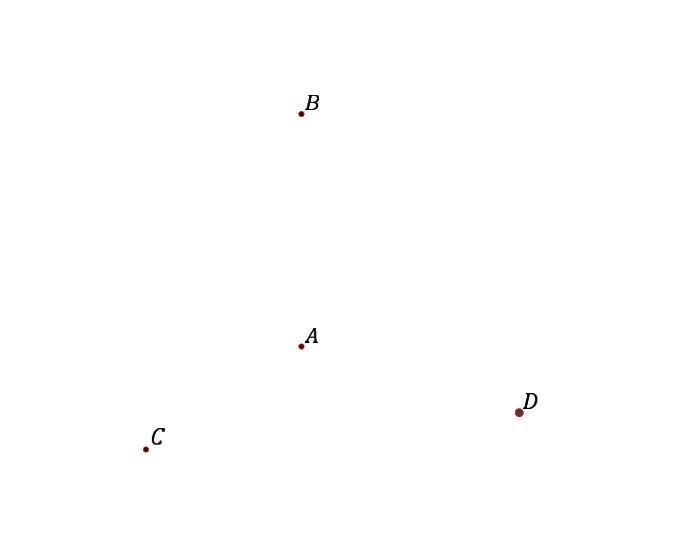
\includegraphics[width=0.6 \linewidth]{img/ch3/4.jpg}}
\end{center}

\pagebreak

\item Создание тетраэдра \texttt{ABCD} по четырём вершинам с помощью \texttt{TetrahedronBuilder}. Параметры билдера --- якоря \texttt{A}, \texttt{B}, \texttt{C}, \texttt{D}\footnote{Квадратными скобками обозначен тот факт, что тело является обёрткой якоря и не имеет билдера.}.

\begin{table}[h!]
\centering
\begin{tabular}{lll}
\texttt{BodyBuilderContainer}                 & \texttt{BodyContainer} & \texttt{AnchorContainer} \\
\texttt{PointBuilder} & \texttt{A}    & \texttt{A}      \\
\texttt{PointBuilder} & \texttt{B}    & \texttt{B}      \\
\texttt{PointBuilder} & \texttt{C}    & \texttt{C}      \\
\texttt{PointBuilder} & \texttt{D}    & \texttt{D}      \\
\cellcolor[HTML]{68CBD0}\texttt{TetrahedronBuilder} & \cellcolor[HTML]{68CBD0}\texttt{ABCD} & \\
\texttt{SphereOutTetrahedronBuilder}          & \cellcolor[HTML]{68CBD0}\texttt{[ABC]} & \cellcolor[HTML]{68CBD0}\texttt{ABC} \\
\texttt{PlaneByPointParallelPolygonBuilder}   & \cellcolor[HTML]{68CBD0}\texttt{[ABD]} & \cellcolor[HTML]{68CBD0}\texttt{ABD} \\
\texttt{TetrahedronSectionBuilder}            & \cellcolor[HTML]{68CBD0}\texttt{[ACD]} & \cellcolor[HTML]{68CBD0}\texttt{ACD} \\
 & \cellcolor[HTML]{68CBD0}\texttt{[BCD]} & \cellcolor[HTML]{68CBD0}\texttt{BCD} \\
 & \cellcolor[HTML]{68CBD0}\texttt{[AB]} & \cellcolor[HTML]{68CBD0}\texttt{AB} \\
 & \cellcolor[HTML]{68CBD0}\texttt{[AC]} & \cellcolor[HTML]{68CBD0}\texttt{AC} \\
 & \cellcolor[HTML]{68CBD0}\texttt{[AD]} & \cellcolor[HTML]{68CBD0}\texttt{AD} \\
 & \cellcolor[HTML]{68CBD0}\texttt{[BC]} & \cellcolor[HTML]{68CBD0}\texttt{BC} \\
 & \cellcolor[HTML]{68CBD0}\texttt{[BD]} & \cellcolor[HTML]{68CBD0}\texttt{BD} \\
 & \cellcolor[HTML]{68CBD0}\texttt{[CD]} & \cellcolor[HTML]{68CBD0}\texttt{CD}
\end{tabular}
\end{table}

\begin{center}
\fbox{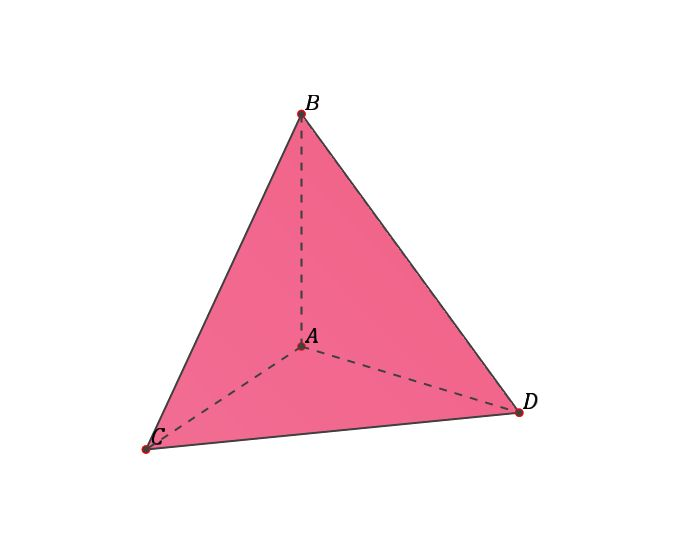
\includegraphics[width=0.6 \linewidth]{img/ch3/5.jpg}}
\end{center}

\pagebreak

\item Создание описанной сферы тетраэдра \texttt{ABCD} с помощью \texttt{SphereOutTetrahedron}. Параметр билдера --- тетраэдр \texttt{ABCD}.

\begin{table}[h!]
\centering
\begin{tabular}{lll}
\texttt{BodyBuilderContainer}                 & \texttt{BodyContainer} & \texttt{AnchorContainer} \\
\texttt{PointBuilder} & \texttt{A}    & \texttt{A}      \\
\texttt{PointBuilder} & \texttt{B}    & \texttt{B}      \\
\texttt{PointBuilder} & \texttt{C}    & \texttt{C}      \\
\texttt{PointBuilder} & \texttt{D}    & \texttt{D}      \\
\texttt{TetrahedronBuilder} & \texttt{ABCD} & \\
\cellcolor[HTML]{68CBD0}\texttt{SphereOutTetrahedronBuilder} & \cellcolor[HTML]{68CBD0}\texttt{sph}              & \\
\texttt{PlaneByPointParallelPolygonBuilder}   & \texttt{[ABC]} & \texttt{ABC} \\
\texttt{TetrahedronSectionBuilder}            & \texttt{[ABD]} & \texttt{ABD} \\
 & \texttt{[ACD]} & \texttt{ACD} \\
 & \texttt{[BCD]} & \texttt{BCD} \\
 & \texttt{[AB]} & \texttt{AB} \\
 & \texttt{[AC]} & \texttt{AC} \\
 & \texttt{[AD]} & \texttt{AD} \\
 & \texttt{[BC]} & \texttt{BC} \\
 & \texttt{[BD]} & \texttt{BD} \\
 & \texttt{[CD]} & \texttt{CD} \\
 & \cellcolor[HTML]{68CBD0}\texttt{[O]}  & \cellcolor[HTML]{68CBD0}\texttt{O} \\
\end{tabular}
\end{table}

\begin{center}
\fbox{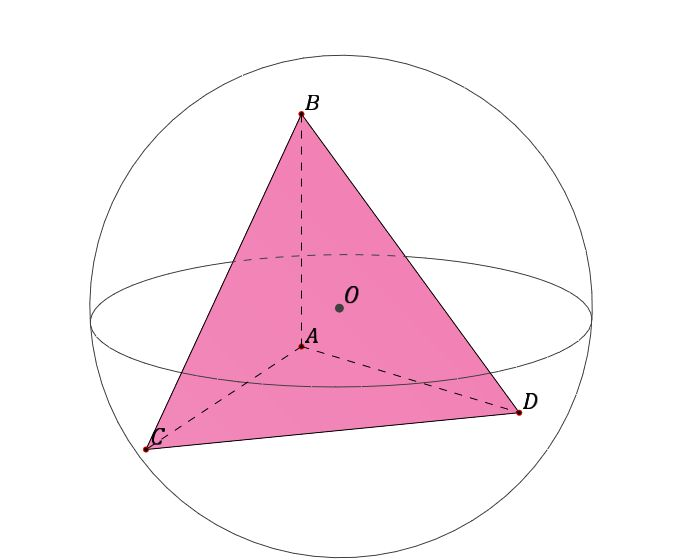
\includegraphics[width=0.6 \linewidth]{img/ch3/6.jpg}}
\end{center}

\pagebreak

\item Построение плоскости, параллельной \texttt{ACD}, проходящей через \texttt{O}, с помощью\\ \texttt{PlaneByPointParallelPolygonBuilder}. Параметры билдера --- якоря \texttt{ACD} и \texttt{O}.

\begin{table}[h!]
\centering
\begin{tabular}{lll}
\texttt{BodyBuilderContainer}                 & \texttt{BodyContainer} & \texttt{AnchorContainer} \\
\texttt{PointBuilder} & \texttt{A}    & \texttt{A}      \\
\texttt{PointBuilder} & \texttt{B}    & \texttt{B}      \\
\texttt{PointBuilder} & \texttt{C}    & \texttt{C}      \\
\texttt{PointBuilder} & \texttt{D}    & \texttt{D}      \\
\texttt{TetrahedronBuilder} & \texttt{ABCD} & \\
\texttt{SphereOutTetrahedronBuilder} & \texttt{sph}              & \\
\cellcolor[HTML]{68CBD0}\texttt{PlaneByPointParallelPolygonBuilder}   & \cellcolor[HTML]{68CBD0}\texttt{pl} & \\
\texttt{TetrahedronSectionBuilder} & \texttt{[ABC]} & \texttt{ABC} \\
 & \texttt{[ABD]} & \texttt{ABD} \\
 & \texttt{[ACD]} & \texttt{ACD} \\
 & \texttt{[BCD]} & \texttt{BCD} \\
 & \texttt{[AB]} & \texttt{AB} \\
 & \texttt{[AC]} & \texttt{AC} \\
 & \texttt{[AD]} & \texttt{AD} \\
 & \texttt{[BC]} & \texttt{BC} \\
 & \texttt{[BD]} & \texttt{BD} \\
 & \texttt{[CD]} & \texttt{CD} \\
 & \texttt{[O]}  & \texttt{O} \\
\end{tabular}
\end{table}

\begin{center}
\fbox{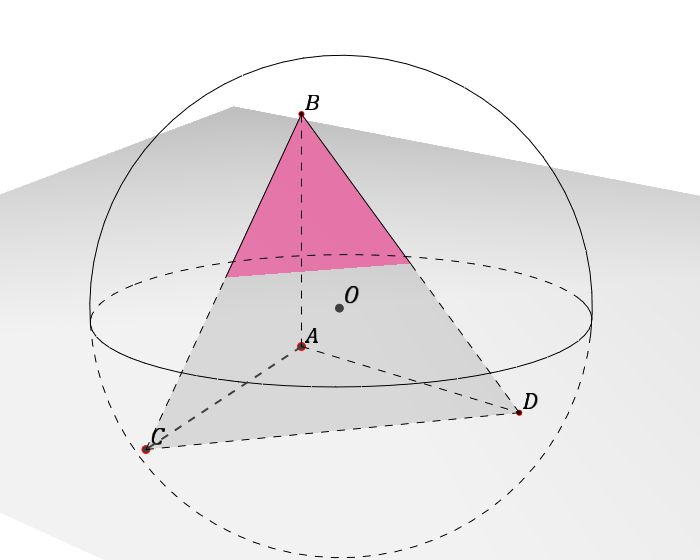
\includegraphics[width=0.6 \linewidth]{img/ch3/7.jpg}}
\end{center}

\pagebreak

\item Построение сечения тетраэдра \texttt{ABCD} плоскостью \texttt{pl} с помощью \texttt{TetrahedronSectionBuilder}. Параметры билдера --- тела \texttt{ABCD} и \texttt{pl}.

\begin{table}[h!]
\centering
\begin{tabular}{lll}
\texttt{BodyBuilderContainer}                 & \texttt{BodyContainer} & \texttt{AnchorContainer} \\
\texttt{PointBuilder} & \texttt{A}    & \texttt{A}      \\
\texttt{PointBuilder} & \texttt{B}    & \texttt{B}      \\
\texttt{PointBuilder} & \texttt{C}    & \texttt{C}      \\
\texttt{PointBuilder} & \texttt{D}    & \texttt{D}      \\
\texttt{TetrahedronBuilder} & \texttt{ABCD} & \\
\texttt{SphereOutTetrahedronBuilder} & \texttt{sph}              & \\
\texttt{PlaneByPointParallelPolygonBuilder} & \texttt{pl} & \\
\cellcolor[HTML]{68CBD0}\texttt{TetrahedronSectionBuilder} & \cellcolor[HTML]{68CBD0}\texttt{$\text{P}_1\text{P}_2\text{P}_3$} & \cellcolor[HTML]{68CBD0}\texttt{$\text{P}_1\text{P}_2\text{P}_3$}\\
 & \texttt{[ABC]} & \texttt{ABC} \\
 & \texttt{[ABD]} & \texttt{ABD} \\
 & \texttt{[ACD]} & \texttt{ACD} \\
 & \texttt{[BCD]} & \texttt{BCD} \\
 & \texttt{[AB]} & \texttt{AB} \\
 & \texttt{[AC]} & \texttt{AC} \\
 & \texttt{[AD]} & \texttt{AD} \\
 & \texttt{[BC]} & \texttt{BC} \\
 & \texttt{[BD]} & \texttt{BD} \\
 & \texttt{[CD]} & \texttt{CD} \\
 & \texttt{[O]}  & \texttt{O} \\
 & \cellcolor[HTML]{68CBD0}\texttt{[$\text{P}_1\text{P}_2$]} & \cellcolor[HTML]{68CBD0}\texttt{$\text{P}_1\text{P}_2$} \\
 & \cellcolor[HTML]{68CBD0}\texttt{[$\text{P}_1\text{P}_3$]} & \cellcolor[HTML]{68CBD0}\texttt{$\text{P}_1\text{P}_3$} \\
 & \cellcolor[HTML]{68CBD0}\texttt{[$\text{P}_2\text{P}_3$]} & \cellcolor[HTML]{68CBD0}\texttt{$\text{P}_2\text{P}_3$} \\
 & \cellcolor[HTML]{68CBD0}\texttt{[$\text{P}_1$]} & \cellcolor[HTML]{68CBD0}\texttt{$\text{P}_1$} \\
 & \cellcolor[HTML]{68CBD0}\texttt{[$\text{P}_2$]} & \cellcolor[HTML]{68CBD0}\texttt{$\text{P}_2$} \\
 & \cellcolor[HTML]{68CBD0}\texttt{[$\text{P}_3$]} & \cellcolor[HTML]{68CBD0}\texttt{$\text{P}_3$} \\
\end{tabular}
\end{table}

\begin{center}
\fbox{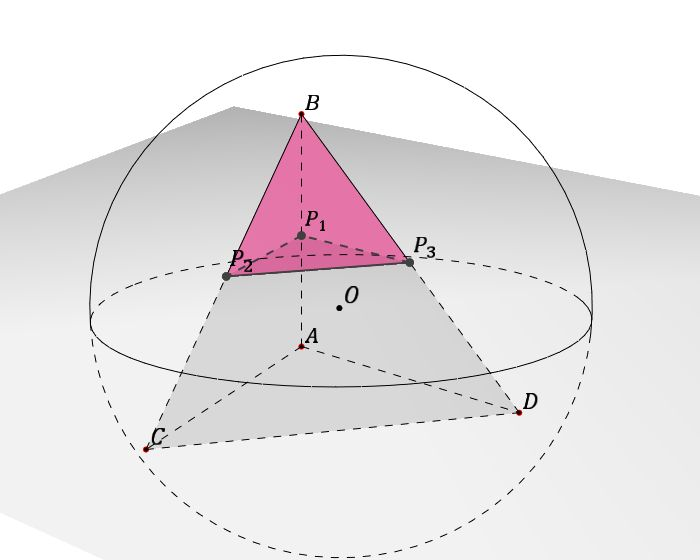
\includegraphics[width=0.6 \linewidth]{img/ch3/8.jpg}}
\end{center}

\end{enumerate}

\chapter{Информация об отображении объектов сцены: пакет \textbf{editor.state}}

\chapter{Математическое ядро: пакет \textbf{geom}}

\chapter{Графика в приложении: пакет \textbf{opengl}}

\chapter{Создание 3D-моделей: пакет \textbf{maquettes}}

\chapter{Фокусировка на объектах}

\chapter{Графический интерфейс. Обзор пакета \textbf{gui}}

\chapter{Позиционирование элементов GUI. Основные виды лейаутов.}

\chapter{Интерактивные режимы построения: пакет \textbf{gui.mode}}

\chapter{Фабрики действий: пакет \textbf{gui.action}}

\chapter{Лицензирование продукта: пакет \textbf{license}}

\chapter{Параметры конфигурации}

За обработку конфигурационных параметров проекта отвечает пакет \texttt{config}. Файлы конфигурации располагаются в домашней папке пользователя. Основной файл конфигурации: \texttt{.3dschooledit/config}. Пользовательские файлы конфигурации: \texttt{.3dschooledit/userconf/$^*$.cfg}

Значения основные конфигурационных параметров загружаются (либо описаны прямо в коде) в класс \texttt{config.Config}.

Параметры конфигурации могут быть:
\begin{itemize}
\item Фискированными внутри кода. Так описываются пути расположения файлов проекта (path parameters).
\item Загружаемые параметры. Такие параметры описываются классом \texttt{ConfigParam}. При их инициализации задаётся значение по умолчанию и адрес в иерархии конфигурационного файла. Например, в коде

\begin{lstlisting}
public static ConfigParam<Font> DEFAULT_FONT = ConfigParamFactory.getFontParam(
          "Main_application_font", "gui.font", true, new Font("Arial", Font.PLAIN, 10));
\end{lstlisting}

создаётся параметр, значением которого является шрифт, т. е. экземпляр класса \texttt{Font}. Строка адреса \texttt{gui.font} означает, что при загрузке из JSON-файла конфигурации значение параметра берётся из подсловаря \texttt{"font"} словаря \texttt{"gui"}.

\begin{lstlisting}
...
"gui": {
	...
	"font": 10;
	...
}
...
\end{lstlisting}

\item Параметры \texttt{UIManager}. Это параметры интерфейса, которые тоже являются загружаемыми, но не хранятся в ходе работы программы, а сразу применяются до создания объектов интерфейса. Из значения хранятся в основном конфигурационном файле по ключам \texttt{"uicolors"} (цветовые параметры) и \texttt{"uistrings"} (строковые параметры).

\item Параметры из properties-файла. Это параметры проекта, связанные с версией сборки. Поскольку версию сборки <<изнутри>> проекта достать не получается, она пишется в процессе сборки в properties-файл. Версию сборки нужно знать для корректной работы сервера обновлений.
\end{itemize}

\section{Загружаемые параметры}

За загрузку, сохранение и хранение загружаемых параметров отвечаем класс \texttt{ConfigParam<T>}. При создании параметра указывается тип его значения (\texttt{T}), <<читаемое>> имя (\texttt{alias}), адрес (\texttt{name}), значение по умолчанию и возможность изменения этого параметра в пользовательской конфигурации (\texttt{mutable}).

Порядок загрузки параметров конфигурации следующий: сначала обрабатывается основной файл (\texttt{config}), из него загружаются все параметры. В основном файле по ключу \texttt{"userconf"} получаем имя пользовательской конфигурации. Если она есть, то ищется файл с соответствующим именем в папке \texttt{userconf/}, после чего параметры загружаются из соответствующего файла, переопределяя значения по умолчанию.

\section{Управление пользовательскими конфигурациями}

В диалоговом окне \texttt{Настройки $\rightarrow$ Конфигурация} пользователю позволяется производить следующие действия.
\begin{itemize}
\item Создание конфигурации. Создаётся новый конфигурационный файл в папке \texttt{userconf/}, в который в формате JSON записываются текущие значения всех загружаемых изменяемых (\texttt{mutable}) параметров приложения.
\item Загрузка существующей конфигурации. Пользователь выбирает конфигурацию из списка доступных и загружает значения параметров из соответствующего файла.
\item Сохранение текущей конфигурации.
\item Удаление конфигурации. Выбранный файл конфигурации удаляется. Если удалённая конфигурация была текущей, то загружается стандартная конфигурация.
\end{itemize}

\section{Временные параметры приложения}
Параметры приложения, которые являются <<временными>>, т. е. их значение не хранится между сессиями работы, хранятся в классе \texttt{config.Temp}.
\end{document}